% !TeX root = ../main-presentation.tex
\begin{frame}
    \frametitle{What are we going to be talking about?}
    \pause
    \centering
    \LARGE
    Digital circuits!

    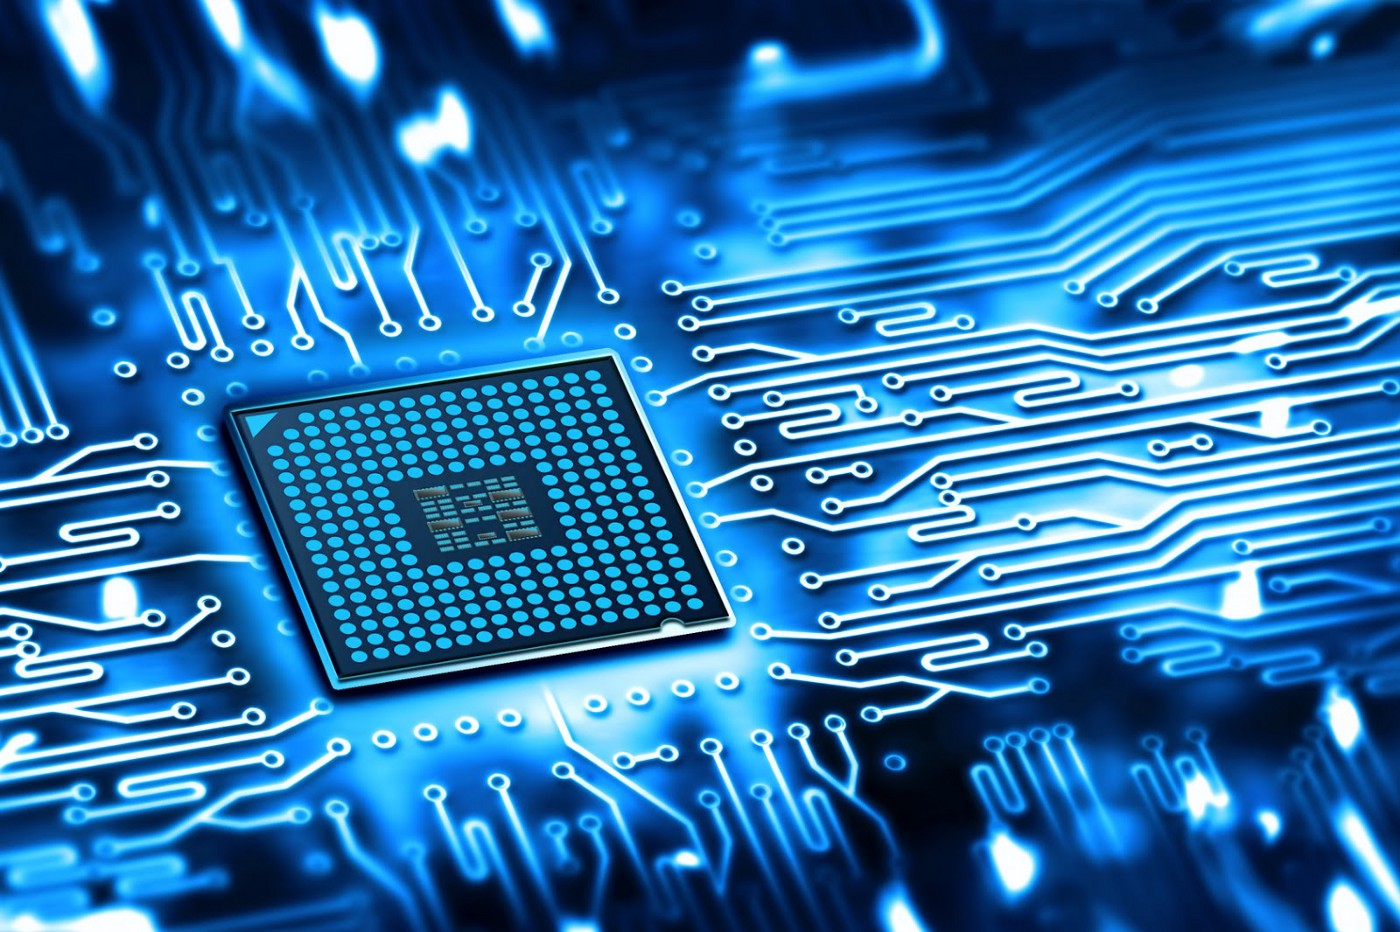
\includegraphics[width=0.6\textwidth]{imgs/circuit}
\end{frame}
\begin{frame}
    \frametitle{What are we going to be talking about?}
    \centering
    \LARGE
    Digital circuits!

    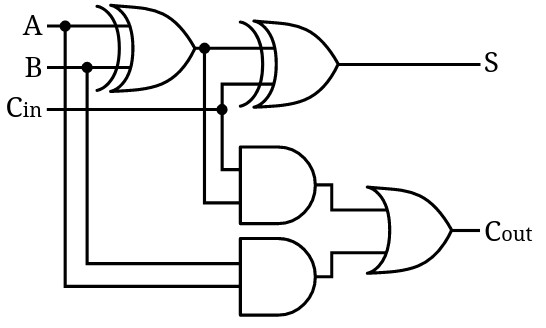
\includegraphics[width=0.6\textwidth]{imgs/adder}
\end{frame}
\begin{frame}
    \frametitle{What are we going to be talking about?}

    \pause

    \centering
    \LARGE
    We want a \alert{compositional} theory of digital circuits.

    \vspace{0.5em}

    \normalsize

    \pause
    \includesvg{imgs/f}
    \pause
    \quad
    \includesvg{imgs/g}
    \pause
    \quad
    \includesvg{imgs/h}


    \pause
    \vspace{1em}

    \raisebox{2em}{\includesvg{imgs/seq}}
    \quad
    \includesvg{imgs/par}
    \quad
    \raisebox{2em}{\includesvg{imgs/trace}}

\end{frame}
\begin{frame}
    \frametitle{But why do we want that?}
    \centering
    \LARGE
    We want to reason \alert{equationally} about circuits.

    \normalsize
    \vspace{2em}

    \pause

    \svg{-0.5}{0.5}{f}
    \quad
    \pause
    \(=\)
    \quad
    \svg{-2}{0.5}{rewrite-l}
    \quad
    \pause
    \(\rightsquigarrow\)
    \quad
    \svg{-2}{0.5}{rewrite-r}
    \quad
    \pause
    \(=\)
    \quad
    \svg{-0.5}{0.5}{g}

\end{frame}
\begin{frame}
    \frametitle{Why all the pictures?}
    \centering
    \LARGE
    \pause
    String diagrams are \alert{good}.

    \normalsize

    \vspace{1em}

    \pause
    \only<3>{\svg{0}{1.25}{string-crossed}}%
    \only<4->{\svg{0}{1.25}{string-uncrossed}}%

    \pause\pause
    \vspace{1em}
    (but these are a little different to the ones Dan and Jamie are using)

\end{frame}